\chapter{Matlab数据及运算}
\thispagestyle{empty}
\section{矩阵的表示}
\subsection{矩阵的建立}
\begin{enumerate}
	\item 直接输入:将矩阵的元素用中括号括起来,按矩阵行的顺序输入各元素,同一行各元素之间用逗号或空格隔开,不同行的元素之间用分号分隔。例如:
	\begin{lstlisting}
>> A = [1, 2, 3; 4, 5, 6; 7, 8, 9]
A = 
		1		2		3
		4		5		6
		7		8		9
	\end{lstlisting}

	\item 利用已建好的矩阵建立更大的模型:大矩阵可由已建好的小矩阵拼接而成。例如:
	\begin{lstlisting}
>> A = [1, 2, 3; 4, 5, 6; 7, 8, 9];
>> B = [-1, -2, -3; -4, -5, -6; -7, -8, -9];
>> C = [A, B; B, A]
C = 
		 1		 2		 3		-1		-2		-3
		 4		 5		 6		-4		-5		-6
		 7		 8		 9		-7		-8		-9
		-1		-2		-3		 1		 2		 3
		-4		-5		-6		 4		 5		 6
		-7		-8		-9		 7		 8		 9
	\end{lstlisting}

\end{enumerate}

\subsection{冒号表达式}
	在Matlab中,利用冒号表达式可以产生行向量,一般格式如下:
	\begin{center}
		\lstinline|e1:e2:e3|
	\end{center}

	其中,\lstinline|e1|为初始值,\lstinline|e2|为步长,\lstinline|e3|为终止值。冒号表达式可以产生一个由\lstinline|e1|开始到\lstinline|e3|结束。以步长\lstinline|e2|自增的行向量。例如:
	\begin{lstlisting}
>> t = 0:1:5
t = 
		0		1		2		3		4		5
	\end{lstlisting}
\warn[
\hspace*{2em} 在冒号表达式中如果省略\lstinline|e2|不写,则默认步长为1.
]

在Matlab中,还可以用\lstinline|linspace|函数产生行向量,其调用格式如下:
\begin{center}
	\lstinline|linspace(a,b,n)|
\end{center}
其中,a和b是生成向量的第一个和最后一个元素,n是元素总数。当n省略时,i懂产生100个元素。例如:
\begin{lstlisting}
>> x = linspace(0, pi, 6)
x =
		0		0.6283		1.2566		1.8850		2.5133		3.1416
\end{lstlisting}

\subsection{矩阵元素的引用}
\begin{enumerate}
	\item 矩阵元素的引用方式
	\begin{enumerate}
		\item 下标引用:下标必须是正整数。例如,将矩阵$\bm{A}$第3行第2列的元素赋值为200(仅改变单个元素的值,其余元素值不改变):
		\begin{lstlisting}
>> A(3, 2) = 200
		\end{lstlisting}
		
		如果给出的行下标或列下标大于原来矩阵的行数和列数,则Matlab自动扩展矩阵的行数和列数,并将扩展后未赋值的的矩阵元素置为0.例如:
		\begin{lstlisting}
>> A[1, 2, 3; 4, 5, 6];
>> A(4, 5) = 10
A =
		1		2		3		0		0
		4		5		6		0		0
		0		0		0		0		0
		0		0		0		0		10
		\end{lstlisting}
		
		\item 序号引用:矩阵元素的序号就是相应元素在内存中的排列顺序,即线性索引号。在Matlab中,矩阵按列储存,即首先储存矩阵的第一列元素,然后储存第二列元素,……,一直到矩阵的最后一列矩阵。例如,矩阵$\bm{A}$的第3号元素为2,即$A(1,2) = 2$:
		\begin{lstlisting}
>> A = [1, 2, 3; 4, 5, 6]
A = 
		1		2		3
		4		5		6
>> A(3)
ans = 
		2
		\end{lstlisting}
		
		\item 序号与下标的转换:对于$m\times n$的矩阵$\bm{A}$来说,$A(i,j)$的序号为$(j-1)*m+i$。\lstinline|sub2ind|与\lstinline|ind2sub|函数实现相互转换。\\
		\lstinline|sub2ind|调用函数:
		\begin{center}
			\lstinline|D = sub2ind(S, I, J)|
		\end{center}
		其中,S表示要转换的矩阵的函数和列数,是行数和列数组成的向量,通常用函数\lstinline|size|获取;I是行下标,J是列下标,D为对应下标元素的序号,其行列数与I、J相同。例如:
		\begin{lstlisting}
>> A = [1:3; 4:6]
A = 
		1		2		3
		4		5		6
>> D = sub2ind(size(A), [1, 2; 2, 2], [1, 1; 3, 2])|
D = 
		1		2
		6		4
		\end{lstlisting}
	
		对于上面的例子,可以解释如下:
		\begin{equation*}
			\begin{bmatrix}
				d_1 & d_2 \\
				d_3 & d_4 \\
			\end{bmatrix}
		\quad \Longrightarrow \quad
			\begin{bmatrix}
				(i_1,j_1) & (i_2,j_2) \\
				(i_3,j_3) & (i_4,j_4) \\
			\end{bmatrix}
		\mbox{下标对应的元素}
		\end{equation*}
	即$A(1,1)$的序号为1,$A(2,1)$的序号为2,$A(2,3)$的序号为6,$A(2,2)$的序号为4.
	
	\lstinline|ind2sub|调用函数
	\begin{center}
		\lstinline|[I, J] = ind2sub(S, D)|
	\end{center}
	其中,S表示要转换的矩阵的行数和列数;D是序号,返回值为序号所对应的行下标和列下标。例如:
\begin{lstlisting}
>> [I, J] = ind2sub([3, 3], [1, 3, 5])
I = 
		1		3		5
J = 
		1		1		2
\end{lstlisting}
	\end{enumerate}

\item 利用冒号表达式获得子矩阵\\
子矩阵是指由矩阵中的一部分元素构成的矩阵。见下表:
\begin{table}[!htb]
	\centering
	\setlength{\tabcolsep}{8mm}{
	\begin{tabular}{cc}
		\toprule
		符号 & 说明\\
		\midrule
		\lstinline|A(i,j)| & $\bm{A}$矩阵第$i$行,第$j$列的元素 \\
		\lstinline|A(i,:)| & $\bm{A}$矩阵第$i$行的全部元素 \\
		\lstinline|A(:,j)| & $\bm{A}$矩阵第$j$列的全部元素 \\
		\lstinline|A(i:i+n,:)| & $\bm{A}$矩阵第$i\thicksim i+n$行的全部元素 \\
		\lstinline|A(:,k:k+m)| & $\bm{A}$矩阵第$k\thicksim k+m$列的全部元素 \\
		\lstinline|A(i:i+n,k:k+m)| & $\bm{A}$矩阵第$i\thicksim i+n$行,且在第$k\thicksim k+m$列的全部元素 \\
		\bottomrule
	\end{tabular}
	}
\end{table}

\newpage
例如:
\begin{lstlisting}
	>> A = [1:5, 6:10, 11:15, 16:20]
	A = 
			1		 2		 3		 4		 5
			6		 7		 8		 9		10
			11		12		13		14		15
			16		17		18		19		20
	>> A(1,:)		% 取A的第一行
	ans = 
			1		2		3		4		5
	>> A(:,2:4)		% 取A的第2,3,4列
	ans = 
			2		 3		 4
			7		 8		 9
			12		13		14
			17		18		19
	>> A(2:3,4:5)		% 取A的第2,3行,第4,5列
	ans = 
			9		10
			14		15
	>> A(2:3,1:2:5)		% 取A的第2,3行,第1,3,5列
	ans =
			6		 8		10
			11		13		15 
\end{lstlisting}
此外,还可以利用一般向量和\lstinline|end|运算符来表示矩阵下标,从而获得子矩阵。\lstinline|end|表示矩阵某一维的末尾元素的下标。例如:
\begin{lstlisting}
>> A = [1:5, 6:10, 11:15, 16:20];
>> A = (end,:)		% 取A的最后一行
ans =
		16		17		18		19		20
>> A([1,4],3:end)		% 取A的第2,3两行中第3列到最后一列的元素
ans = 
		 3		 4		 5
		18		19		20	
\end{lstlisting}

\item 利用空矩阵删除矩阵的元素\\
空矩阵是指没有任何元素的矩阵,即在建立矩阵时,中括号中为空。\\
调用格式为:
\begin{center}
	\lstinline|X = [ ]|
\end{center}
将某些元素从矩阵中删除,采用将其置为空矩阵的方法是一种有效的方法,例如:
\begin{lstlisting}
>> A = [1, 2, 3, 0, 0; 7, 0, 9, 2, 6; 1, 4, -1, 1, 8]
A = 
		1		2		3		0		0
		7		0		9		2		6
		1		4		-1		1		8
>> A(:, [2, 4]) = [ ]
A = 
		1		3		0
		7		9		6
		1		-1		8
\end{lstlisting}

\item 改变矩阵的形状\\
\lstinline|reshape(A, m, n)|函数在矩阵总元素保持不变的前提下,将矩阵$\bm{A}$重新排成$m \times n$的二维矩阵。例如:
\begin{lstlisting}
>> x = [23, 45, 65, 34, 65, 34, 98, 45, 78, 65, 43, 76];
>> y = reshape(x, 3, 4)
y = 
		23		34		98		65
		45		65		45		43
		65		34		78		76
>> z = reshape(y, 2, 6)
z = 
		23		65		65		98		78		43
		45		34		34		45		65		76
\end{lstlisting}
\warn[
\quad \lstinline|reshape|函数只是改变原矩阵的行数和列数,即改变其逻辑结构,但并不改变原矩阵的元素个数和其储存顺序。
]
\lstinline|A(:)|将矩阵$A$的每一列元素堆叠起来,成为一个列向量,从而改变了矩阵的形状。例如:
\begin{lstlisting}
>> A = [-45, 65, 71; 27, 35, 91]
A = 
		-45		65		71
		27		35		91
>> B = A(:)
B =
		-45
		27
		65
		35
		71
		91
\end{lstlisting}
\end{enumerate}

\section{变量及其操作}

\subsection{变量的命名}
\begin{itemize}
	\item 在Matlab中,变量名是以字母开头、后接字母、数字或下画线的字符序列,最多63个字符。
	\item 在Matlab中,变量名区分字母的大小写。例如:\lstinline|example, Exmple, EXAMPLE|是3个不同的变量。
\end{itemize}
\warn[
\quad Matlab提供的标准函数名以及命令名一般都是小写字母。例如求矩阵$\bm{A}$的逆用\lstinline|inv(A)|,不能写成\lstinline|Inv(A), INV(A)|,否则会出错。
]

\subsection{变量的赋值}
变量的赋值有以下下两种方式:
\begin{enumerate}[\hspace{3em}$\bullet$]
	\item 变量 = 表达式\\
	这种方式是把表达式的值直接赋值给变量。
	\item 表达式\\
	这种方式是把表达式的值赋值给Matlab预定义的变量\lstinline|ans|中。
\end{enumerate}

当赋值命令的结果不需要在命令行窗口输出的时候,通常在赋值语句后面加上\lstinline|;|。

\examples 计算表达式$\dfrac{5+\cos 47\degree}{1+|x-y|}$的值,并将结果赋值给变量$z$,然后显示计算结果。其中$\displaystyle x = \sqrt{7} - 2\i, y = \e^{\frac{\pi}{2}}$.\vspace{0.5em}

\begin{lstlisting}
>> x = sqrt(7) - 2i;
>> y = exp(pi / 2);
>> z = (5 + cos(47 * pi / 180) / (1 + abs(x - y)))
z =
		1.4395
\end{lstlisting}

\subsection{预定义变量}
Matlab常用的自定义变量如下表:
\begin{table}[!htb]
	\centering
	\setlength{\tabcolsep}{7mm}{
		\begin{tabular}{cccc}
			\toprule
			符号 & 说明 & 符号 & 说明\\
			\hline
			\lstinline |ans| & 计算结果的默认赋值变量 & \lstinline|nargin| & 函数输入参数的个数\\
			\lstinline|eps| & 机器零阈值 & \lstinline|nargout| & 函数输出参数的个数\\
			\lstinline|pi| & 圆周率$\pi$的近似值 & \lstinline|realmax| & 最大正实数\\
			\lstinline|i, j| & 虚数单位 & \lstinline|realmin| & 最小正实数\\
			\lstinline|inf, Inf| & 无穷大,如$1/0$的结果 & \lstinline|lasterr| & 存放最新的错误消息\\
			\lstinline|NaN, nan| & 非数,如$0/0,$inf$ / $inf的结果 & \lstinline|lastwarn| & 存放最新的警告消息\\
			\bottomrule
		\end{tabular}
	}
\end{table}

\newpage
\warn[
\quad 对于Matlab预定义的变量,在使用时尽量避免对这些变量重新赋值。对于我们循环常用的$i,j$来说,进行复数运算我们要注意:对复数赋值使用\lstinline|3 + 4i|这样的记法,而不是\lstinline|3 + 4 * i|的记法,下面举例说明不同之处。
]
\begin{lstlisting}
>> i = 10;
>> 3 + 4i
ans =
		3.0000 + 4.0000i
>> 3 + 4 * i
ans =
		43
\end{lstlisting}

\subsection{变量的管理}
\begin{enumerate}
	\item 内存变量的删除和修改\\
	MATLAB工作区窗口专门用于内存变量的管理。在工作区窗口中可以显示所有内存变量的
	属性。当选中某些变量后,选择右键快捷菜单中的“删除”命令,就能清除这些变量。当选中某
	个变量后,双击该变量或选择右键快捷菜单中的“打开所选内容”命令,将进入变量编辑器。通过变量编辑器可以直接观察变量中的具体元素,也可以修改变量中的具体元素。\\
	通常,对于较大矩阵的输入,可以采用变量编辑器,操作方法如下:
	\begin{enumerate}[(1)]
		\item 在工作区窗口的右键快捷键中选择“新建”命令,并给变量命名。
		\item 在工作区中双击该变量,打开变量编辑器。
		\item 在变量编辑器的空白表格中填写元素值,表格的每一个方格对应矩阵的一个元素。
	\end{enumerate}
	命令行窗口删除、查看变量的函数如下表:
	\begin{table}[!htb]
		\centering
		\setlength{\tabcolsep}{9mm}{
			\begin{tabular}{cc}
				\toprule
				命令 & 说明\\
				\midrule
				\lstinline|clear| & 删除工作区的所有变量 \\
				\lstinline|who| & 输出所有变量的变量名 \\
				\lstinline|whos| & 输出所有变量的变量名、大小、所占字节数及数据类型等信息 \\
				\bottomrule
			\end{tabular}
		}
	\end{table}
\vspace*{-1em}
\begin{lstlisting}
	>> who
	Your variables are:
	a	x	y	z
	>> whos
	Name			Size					Bytes		Class			Attributes
	a				2*6					  96		double
	x				1*1						8		double
	y				1*1						8		double
	z				1*1						8		double
\end{lstlisting}
\item 内存变量文件\\
利用Mat文件可以把当前Matlab工作区中的一些有用变量长久的储存下来。Mat文件是Matlab保存数据的一种标准的二进制格式文件,扩展名一定是\lstinline|.mat|。Mat文件的生成和载入由\lstinline|save|和\lstinline|load|来完成。\\
常用格式如下:
\par \quad \quad  \lstinline|save [file name] [variable names] [-append] [-ascii]|
\par \quad \quad \lstinline|load [file name] [variable names] [-ascii]|
\par 其中,
\begin{itemize}
	\item \lstinline|file name|是储存Mat文件的文件名(可以带路径,但不需要带后缀名\lstinline|.mat|)。
	\item \lstinline|variable names|是指变量名表,个数不限,只要工作区内存或文件中存在即可,变量名之间以空格分隔。\textbf{当变量名省略时,保存或载入全部变量。}
	\item \lstinline|-ascii|选项使文件以ASCII格式处理,省略该选项时文件将以二进制格式储存。
	\item \lstinline|-append|选项在\lstinline|save|命令中控制将变量追加到Mat文件中。
\end{itemize}
\begin{lstlisting}
>> save d:\example\mydata a x
>> load d:\example\mydata
\end{lstlisting}
\end{enumerate}

\section{Matlab常用的内部函数}
\subsection{常用的数学函数}
\begin{table}[!htb]
	\centering
	\setlength{\tabcolsep}{6mm}{
		\begin{tabular}{cccc}
			\toprule
			函数名 & 功能 & 函数名 & 功能\\
			\hline
			\lstinline |sin (sind)| & 正弦函数,输入值为弧度(角度) & \lstinline|abs| & 绝对值函数\\
			\lstinline|cos (cosd)| & 余弦函数,输入值为弧度(角度) & \lstinline|rem| & 求余函数\\
			\lstinline|tan (tand)| & 正切函数,输入值为弧度(角度) & \lstinline|mod| & 求模函数\\
			\lstinline|asin (asind)| & 反正弦函数,输入值为弧度(角度) & \lstinline|fix| & 向零方向取整\\
			\lstinline|acos (acosd)| & 反余弦函数,输入值为弧度(角度) & \lstinline|floor| & 不大于自变量的最大函数\\
			\lstinline|atan (atand)| & 反正切函数,输入值为弧度(角度) & \lstinline|ceil| & 不小于自变量的最小整数\\
			\lstinline|sinh (asinh)| & 双曲正弦函数(反双曲正弦函数) & \lstinline|round| & 四舍五入到最邻近的整数\\
			\lstinline|cosh (acosh)| & 双曲余弦函数(反双曲余弦函数) & \lstinline|sign| & 符号函数\\
			\lstinline|tanh (atanh)| & 双曲正切函数(反双曲正切函数) & \lstinline|gcd| & 最大公约数\\
			\lstinline|sqrt| & 平方根函数 & \lstinline|lcm|  & 最小公倍数\\
			\lstinline|log| & 自然对数函数 & \lstinline|factorial|  & 阶乘\\
			\lstinline|log10| & 常用对数函数 & \lstinline|isprime|  & 判断是否为素数\\
			\lstinline|log2| & 以2为底的对数函数 & \lstinline|primes|  & 生成素数列表\\
			\lstinline|exp| & 自然指数幂数 & \lstinline|perms|  & 生成所有排列\\
			\lstinline|pow2| & 2的幂数 & \lstinline|randperms|  & 生成任意排列\\
			\bottomrule
		\end{tabular}
	}
\end{table}

% 流程图定义基本形状
\tikzstyle{ellipse}=[draw, rectangle, minimum width=2.8em, rounded corners=6pt,line width=0.5pt]% minimum height=1.5em, fill=red!20
\tikzstyle{pxsbx}=[trapezium, trapezium left angle=75, trapezium right angle=105, minimum width=3em, text centered, draw = black, fill=white,line width=0.5pt]
\tikzstyle{lingxing}=[draw,diamond,shape aspect=3,inner sep = 0.4pt,thick,font=\itshape,line width=0.5pt]%,minimum size=8mm
\warn[
1. 取整函数的区别\\
\hspace*{2em} 常用的取整函数有:\lstinline|fix, floor, ceil, round|。其中,\lstinline|round|等价于四舍五入。设$a$为最靠近$x$的正整数($|x| \ge a$),则其余3个函数的区别如图\ref{JT}.

{
	\vspace*{-1.5em}
\begin{center}
	\captionof{figure}{\lstinline|fix, floor, ceil|取整函数对区别示意图}
	\vspace{1em}
	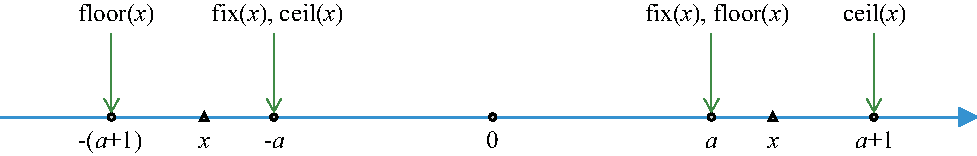
\includegraphics[width=0.8\linewidth]{pic/C-1/箭头.pdf}
	\label{JT}
\end{center}
}

2. 求余运算和求模运算的区别如图\ref{求余求模}.
{
\captionof{figure}{求余运算和求模运算的算法示意图}
\label{求余求模}
\begin{center}
	\begin{tikzpicture}[node distance=1.2cm]
		%定义流程图具体形状
		\node(A)[minimum height=0cm,draw, node distance=1cm,inner sep=8pt] {\quad 输入$a,b$\quad \quad };
		\node (B) [minimum height=0cm,draw, below of=A,node distance=1.5cm,inner sep=8pt] {\quad   求整数商$c=a/b$\quad \quad  };
		\node (C) [minimum height=0cm,draw, below of=B,node distance=1.5cm,inner sep=8pt] {\quad   $r = a-c*b$\quad \quad  };
		\node (D1) [minimum height=0cm,draw, below of=C,node distance=2cm,inner sep=8pt,xshift = 4cm] {\quad  \lstinline|ans = floor(r)|\quad \quad  };
		\node (D2) [minimum height=0cm,draw, below of=C,node distance=2cm,inner sep=8pt,xshift = -4cm] {\quad  \lstinline|ans = fix(r)|\quad \quad  };
		
		%连接具体形状
		\draw[arrows={-Stealth[scale=0.8]}](A) -- (B) ;
		\draw[arrows={-Stealth[scale=0.8]}](B) -- (C) ;
		%\draw[arrows={-Stealth[scale=0.8]}](A) --+(0,-1cm) node[midway,right=1.5cm,above=-0.3cm]{N}|-(A1) ;
		\draw[arrows={-Stealth[scale=0.8]}](C) --+(0,-1.2cm)node[midway,right=2cm,above=-0.3cm]{取模函数\lstinline|mod|}|-+(4cm,-1.2cm) -- (D1);
		\draw[arrows={-Stealth[scale=0.8]}](C) --+(0,-1.2cm)node[midway,right=-2cm,above=-0.3cm]{取余函数\lstinline|rem|}|-+(-4cm,-1.2cm) -- (D2);
	\end{tikzpicture}
\end{center}
}
]

\subsection{矩阵的超越函数}
Matlab还提供了一些直接作用于矩阵的超越函数,\textbf{这些函数名都在上述内部函数名之后缀以m,并规定输入参数\lstinline|A|必须是方阵。}
常见的超越函数如下表:
	\begin{table}[!htb]
	\centering
	\setlength{\tabcolsep}{10mm}{
		\begin{tabular}{cc}
			\toprule
			函数 & 说明\\
			\midrule
			\lstinline|sqrtm(A)| & 计算矩阵$\bm{A}$的平方根,即$\sqrt{\bm{A}}\cdot \sqrt{\bm{A}} = \bm{A}$ \\
			\lstinline|logm(A)| & 计算矩阵$\bm{A}$的自然对数 \\
			\lstinline|expm(A)| & 计算矩阵指数$\e^{\bm{A}}$ \\
			\bottomrule
		\end{tabular}
	}
\end{table}

\textbf{普通矩阵函数}
\par \lstinline|funm(A, @fun)|对方阵$\bm{A}$计算由\lstinline|fun|定义的矩阵函数值。例如,当\lstinline|fun|取\lstinline|exp|时,\lstinline|funm(A, @exp)|可以计算矩阵$\bm{A}$的指数,与\lstinline|expm(A)|的计算结果一致:
\begin{lstlisting}
>> A = [2, -1; 1, 0];
>> funm(A, @exp)
ans = 
		5.4366		-2.7183
		2.7183		0.0000
>> expm(A)
ans = 
		5.4366		-2.7183
		2.7183				 0
\end{lstlisting}
\warn[
	\hspace*{2em}\lstinline|funm(A, @fun)|可以使用的函数有:\lstinline|exp, log, sin, cos, sinh, cosh|等,\textbf{但求矩阵的的平方根只能用\lstinline|sqrtm(A)|}。
]

\section{Matlab 运算}
\subsection{算术运算}
Matlab运算是在矩阵意义下进行的,单个数据的算术运算只是一种特例。运算符号如下表:
	\begin{table}[!htb]
	\centering
	\setlength{\tabcolsep}{6mm}{
		\begin{tabular}{ccc}
			\toprule
			运算符 & 说明 & 适用条件\\
			\midrule
			\lstinline|A + B| & 矩阵的加法运算 & 矩阵$\bm{A}, \bm{B}$同型\\
			\lstinline|A - B|  & 矩阵的减法运算 & 矩阵$\bm{A}, \bm{B}$同型 \\
			\lstinline|A * B|  & 矩阵的乘法运算 & 矩阵$\bm{A}$的列数等于矩阵$\bm{B}$的行数 \\
			\lstinline|A \ B| & 矩阵$\bm{A}$左除矩阵$\bm{B}$,即$\bm{A}$的逆左乘$B$矩阵 &  矩阵$\bm{A}, \bm{B}$同型 \\
			\lstinline|B / A| & 矩阵$\bm{B}$右除矩阵$\bm{A}$,即$\bm{B}$的逆右乘$A$矩阵 &  矩阵$\bm{A}, \bm{B}$同型 \\
			\lstinline|A ^ x| & 矩阵$\bm{A
			}$的$x$次幂 &  矩阵$\bm{A}$是方阵 \\
			\lstinline|A .* B| & 矩阵$\bm{A}$和矩阵$\bm{B}$单个元素之间对应相乘 &  矩阵$\bm{A}, \bm{B}$同型 \\
			\lstinline|A .\ B| & 矩阵$\bm{A}$除以矩阵$\bm{B}$的对应元素 &  矩阵$\bm{A}, \bm{B}$同型 \\
			\lstinline|B ./ A| & 与\lstinline|A .\ B|等价 &  矩阵$\bm{A}, \bm{B}$同型 \\
			\lstinline|A .^ B| & 矩阵$\bm{A}$和矩阵$\bm{B}$单个元素之间对应取幂 &  矩阵$\bm{A}, \bm{B}$同型 \\
			\bottomrule
		\end{tabular}
	}
\end{table}

\warn[
点运算和乘除法的区别\\
\hspace*{2em}点运算是指两个矩阵对应元素进行基本的算术运算,而乘除法运算是矩阵特有的乘除法运算。尤其是乘法,点乘和乘法对矩阵的要求不一样,容易出错。下面举个例子。
]

\begin{lstlisting}
>> x = 0.1:0.3:1;

>> y = sin(x) * cos(x)
Error using  * 
Incorrect dimensions for matrix multiplication. Check that the number of columns in the first
matrix matches the number of rows in the second matrix. To perform elementwise multiplication, 
use '.*'.

>> y = sin(x) .* cos(x)
y =
		0.0993		0.3587		0.4927		0.4546
\end{lstlisting}

\subsection{关系运算}
Matlab提供了多种关系运算符及函数如下:
\begin{table}[!htb]
	\centering
	\setlength{\tabcolsep}{8mm}{
		\begin{tabular}{ccl}
			\toprule
			运算符 & 函数 & \hspace*{12em}说明\\
			\midrule
			\lstinline|<| & \lstinline|lt| & 小于\\
			\lstinline|<=| & \lstinline|le| & 小于等于\\
			\lstinline|>| & \lstinline|gt| & 大于\\
			\lstinline|>=| & \lstinline|ge| & 大于等于\\
			\lstinline|==| & \lstinline|eq| & 等于\\
			\lstinline|~=| & \lstinline|ne| & 不等于\\
			—— & \lstinline|all| & 若向量的所有元素非零,则结果为1,否则为0\\
			—— & \lstinline|any| & 若向量中任何一个元素非零,则结果为1,否则为0\\
			—— & \lstinline|exsit| & 若变量在工作区是否存在,如果存在,结果为1,否则为0\\
			—— & \lstinline|find| & 找出向量或矩阵中非零元素的位置\\
			—— & \lstinline|isempty| & 若被查矩阵是空矩阵,则结果为1,否则为0\\
			—— & \lstinline|isinf| & 若元素是\lstinline|inf|,则结果矩阵相应位置元素取1,否则取0\\
			—— & \lstinline|isnan| & 若元素是\lstinline|nan|,则结果矩阵相应位置元素取1,否则取0\\
			—— & \lstinline|isfinite| & 若元素大小有限,则结果矩阵相应位置元素取1,否则取0\\
			—— & \lstinline|isinteger| & 若元素变量是整型,则结果取1,否则取0\\
			—— & \lstinline|isnumeric| & 若元素变量是数值型,则结果取1,否则取0\\
			—— & \lstinline|isreal| & 若元素变量是实数,则结果取1,否则取0\\
			—— & \lstinline|isfloat| & 若元素变量是浮点型,则结果取1,否则取0\\
			\bottomrule
		\end{tabular}
	}
\end{table}

关系运算符的运算法则如下:
\begin{enumerate}[\hspace*{3em}$\bullet$]
	\item 结果显示:成立为\lstinline|1|,不成立为\lstinline|0|.
	\item 标量比标量:两数直接按关系符运算。
	\item 矩阵比矩阵(要求同型):相同位置的元素一一按关系符运算,每个元素的位置得到一个结果,最后输出一个结果矩阵(与比较矩阵同型)。
	\item 标量比矩阵:标量与矩阵的每一个元素一一按关系符运算,每个元素的位置得到一个结果,最后输出一个结果矩阵(与比较矩阵同型)。
\end{enumerate}

\examples 产生5阶随机方阵$\bm{A}$,其元素为$[10,90]$区间的随机整数,然后判断$\bm{A}$元素是否能被3整除。
\begin{lstlisting}
>> A = fix((90-10+1) * rand(5) + 10)
A = 
		75		17		22		21		63
		83		32		88		44		12
		20		54		87		84		78
		83		87		49		74		85
		61		88		74		87		64
P = rem(A, 3) == 0			% 等价于 P = eq(rem(A, 3), 0)
P =
		1		0		0		0		1
		0		0		0		0		1
		0		1		1		1		1
		0		1		0		0		0
		0		0		0		1		0
\end{lstlisting}

\subsection{逻辑运算}
Matlab提供了多种关系运算符及函数如下:
\begin{table}[!htb]
	\centering
	\setlength{\tabcolsep}{7mm}{
		\begin{tabular}{ccl}
			\toprule
			运算符 & 函数 & \hspace*{10em}说明\\
			\midrule
			\lstinline|a & b| & \lstinline|and(a, b)| & 与:当$a,b$全为非零时,结果为1,否则为0\\
			\lstinline|a | | \lstinline| b| & \lstinline|or(a, b)| & 或:当$a,b$中只要有一个非零,结果为1,否则为0\\
			\lstinline| ~a | & \lstinline|not(a, b)| & 非:当$a$是零时,结果为1,否则为0\\
			—— & \lstinline|xor(a,b)| & 异或:当$a,b$当值不同时,结果为1,否则为0\\
			\bottomrule
		\end{tabular}
	}
\end{table}

逻辑运算的运算法则
\begin{enumerate}[\hspace*{3em}$\bullet$]
	\item 标量和标量:两数直接按逻辑运算符运算。
	\item 矩阵和矩阵(要求同型):相同位置的元素一一按逻辑运算符运算,每个元素的位置得到一个结果,最后输出一个结果矩阵(与比较矩阵同型)。
	\item 标量和矩阵:标量与矩阵的每一个元素一一按逻辑运算符运算,每个元素的位置得到一个结果,最后输出一个结果矩阵(与比较矩阵同型)。
\end{enumerate}
例如:
\begin{lstlisting}
>> A = [4, 65, -54, 0 ,6];
>> B = [0, 5, 3, 2, -6];
>> A & B
ans = 
		0		1		1		0		1
>> xor(A > 10 , B < 10)
ans = 
		1		0		1		1		1
\end{lstlisting}
\warn[
运算的优先级\\
\hspace*{2em} 算术运算 > 关系运算 > 逻辑运算
]

\section{字符串}
\subsection{字符串的表示}
\begin{itemize}
	\item \textbf{在Matlab中,字符串是用单引号括起来的字符序列,特别的,单引号字符是用两个的单引号来表示。}
	例如:
\begin{lstlisting}
>> str = ' I ''m a teacher. '
str =
		I 'm a teacher.
\end{lstlisting}
	\item \textbf{Matlab将一个字符串当作一个行向量,每个元素对应一个字符,其引用方法和数值矩阵相同。}例如:
\begin{lstlisting}
>> A = 'abcdefg';
>> A(1:3)
ans =
		abc
\end{lstlisting}

	\item 在各行字符数相等的情况下(不相等可以用空格补齐),可以建立字符串矩阵。例如:
	\begin{lstlisting}
>> ch = ['abcdef'; '12345 ']
ch =
		'abcdef'
		'12345 '
>> ch(2, 3)
ans =
		3
	\end{lstlisting}
\end{itemize}

\examples 建立一个字符串向量,然后对该向量做如下处理。
\begin{enumerate}[\hspace*{1em}(1)]
	\item 取1~5个字符组成对子字符串。
	\item 将字符串倒序。
	\item 将字符串中的小写字母变成相应的大写字母,其余字符不变。
	\item 统计字符串中小写字母的个数。
\end{enumerate}
\begin{lstlisting}
>> ch = 'Sun Yat-sen University';
>> subch = ch(1:5)			% 取子字符串
subch =
		'Sun Y'
>> revch = ch(end:-1:1)			% 字符串倒序
revch =
		'ytisrevinU nes-taY nuS'
>> k = find(ch >= 'a' & ch <= 'z');			% 找小写字母的位置
>> ch(k) = ch(k) - ('a' - 'A')			% 将小写字母换成大写字母
ch =
		'SUN YAT-SEN UNIVERSITY'
>> length(k)			% 小写字母的个数
ans =
		16
\end{lstlisting}

\subsection{字符串的操作}
常见的字符串操作见下表:
\begin{table}[!htb]
	\centering
	\setlength{\tabcolsep}{6mm}{
	\begin{tabular}{cll}
		\toprule
		功能 & \hspace*{4em}函数名 & \hspace*{9em}说明\\
		\midrule
		字符串的执行 & \lstinline|eval| & 把字符串的内容作为对应的Matlab命令来执行\\
		\hline
		\multirow{6}*{字符串的转换} & \lstinline|abs, double| & 获取字符串矩阵对应的ASCII码数值矩阵\\
		& \lstinline|char| & 把ASCII码矩阵转换成字符串矩阵\\
		& \lstinline|setstr| & 把单个ASCII码值转换成对应的字符\\
		& \lstinline|str2num, str2double| & 把数字字符转换成数值\\
		& \lstinline|num2str| & 把数值转换成字符串\\
		& \lstinline|int2str| & 把整数转换成字符串\\
		\hline
		\multirow{2}*{字符串的连接} & \lstinline|['str1', str2]| & 将若干个字符串连接起来\\
		& \lstinline|strcat| & 将若干个字符串连接起来\\
		\hline
		\multirow{7}*{字符串的比较} & 关系运算符 & \makecell[l]{\textbf{当两个字符串拥有相同的长度时,}关系运算符对\\每个字符对ASCII码进行比较,最后输出一个数\\值向量,其元素为对应对比较结果}\\
		& \lstinline|strcmp(s1, s2)| & 比较字符串\lstinline|s1, s2|是否相等,相等为1,否则为0\\
		& \lstinline|strcmp(s1, s2, n)| & 比较前n个字符是否相等,相等为1,否则为0\\
		& \lstinline|strcmpi(s1, s2)| & \makecell[l]{忽略字符串大小写的情况下,\\
			比较字符串\lstinline|s1, s2|是否相等,相等为1,否则为0}\\
		& \lstinline|strcmp(s1, s2, n)| & \makecell[l]{忽略字符串大小写的情况下,\\
			比较前n个字符是否相等,相等为1,否则为0}\\
		\hline
		字符串的查找 & \lstinline|findstr(s1, s2)| & 返回短字符串在长字符串中的开始位置。\\
		\hline
		字符串的替换 & \lstinline|strrep(s1, s2, s3)| & 将字符串的\lstinline|s1|中的所有子字符串\lstinline|s2|替换成\lstinline|s3|\\
		\bottomrule
	\end{tabular}
}
\end{table}

\newpage
\begin{lstlisting}
% 字符串的执行
>> t = pi;
>> m = ' [t, sin(t), cos(t)] '
>> y = eval(t)
y =
		3.1416		0.0000		-1.0000

% 字符串的转换
>> s1 = 'MATLAB'
>> a = abs(s1)
a =
		77		65		84		76		65		66
>> char(a + 32)
ans =
		matlab
		
% 字符串的连接
>> f = 70;
>> c = (f - 32) / 1.8;
>> [ 'Room temperature is ', num2str(c), ' degrees C.']
ans =
		Room temperature is 21.1111 degrees C.
>> strcat('ss', 'ff', 'DD', '1234')
ans =
		ssffDD1234
		
% 字符串的比较
>> 'www0' >= 'W123'
ans =
		1		1		1		0
>> strcmp('www0', 'W123')
ans =
		0
>> strncmpi('www0', 'W123')
ans =
		1

% 字符串的查找
>> p = findstr('This is a test!', 'is')
p = 
		3		6
		
% 字符串的替换
>> result = strrep('This is a test!', 'test', 'class')
result =
		This is a class!
\end{lstlisting}

\section{结构数据和单元数据}
\subsection{结构数据}
\begin{enumerate}
	\item 结构矩阵的建立与引用
	\begin{itemize}
		\item 结构矩阵的元素可以是不同的数据类型,它能将\textbf{一组具有不同属性的数据}纳入到一个统一的变量名下进行管理。
		\item 建立一个结构矩阵的表达式:
		\begin{center}
			\lstinline|结构矩阵元素.变量名 = 表达式|
		\end{center}
	其中,表达式应理解为矩阵表达式,而且,结构矩阵元素的成员也可以是结构数据。
	\item 引用结构矩阵
	\begin{itemize}
		\item 引用结构矩阵的非矩阵成员:显示其值
		\item 引用结构矩阵的矩阵成员:仅显示其大小参数而不显示其具体内容
		\item 引用结构矩阵的元素:显示成员名和它的值
		\item 引用结构矩阵:只显示结构矩阵的大小参数和成员名
	\end{itemize}
	\item 示例代码
	\begin{lstlisting}
>> a(1).x1 = 10; a(1).x2 = 'liu'; a (1).x3 = [11, 21; 34, 78];
>> a(2).x1.x11 = 90; a(2).x1.x12 = 12; a(2).x1.x13 = 30; a(2).x2 = 'wang'; a(2).x3 = [34, 191; 27, 578];
>> a(3).x1 = 14; a(3).x2 = 'cai'; a(3).x3 = [13, 890; 67, 231];
>> a(2).x3			% 引用结构矩阵元素a(2)的成员x3
ans = 
    	34   191
		27   578
>> a(2)				% 引用结构矩阵元素a(2)
ans = 
	包含以下字段的 struct:
		x1: [1×1 struct]
		x2: 'wang'
		x3: [2×2 double]
>> a					% 引用结构矩阵a
a =
	包含以下字段的 1×3 struct 数组:
		x1
		x2
		x3
	\end{lstlisting}
	\end{itemize}
\item 结构成员的修改
\begin{itemize}
	\item 增加成员:\\
	\lstinline|		>> a(1).x4 = '410075'|
	\item 删除成员:\\
	\lstinline|		>> a = rmfield(a, 'x4')|
\end{itemize}
\end{enumerate}


